\chapter{Introduction}
% \begin{singlespace}
% \emph{The text and ideas presented in this section were originally proposed by the NASA Innovative Advance Concepts (NIAC) solicitation submitted in 2013 and granted in 2014~\cite{NIACfinalreport}.
% My dissertation proposal draws heavily from this project and was funded by this grant.}
% \end{singlespace}

\section{Motivation}

\begin{figure}[htb]
   \centering
   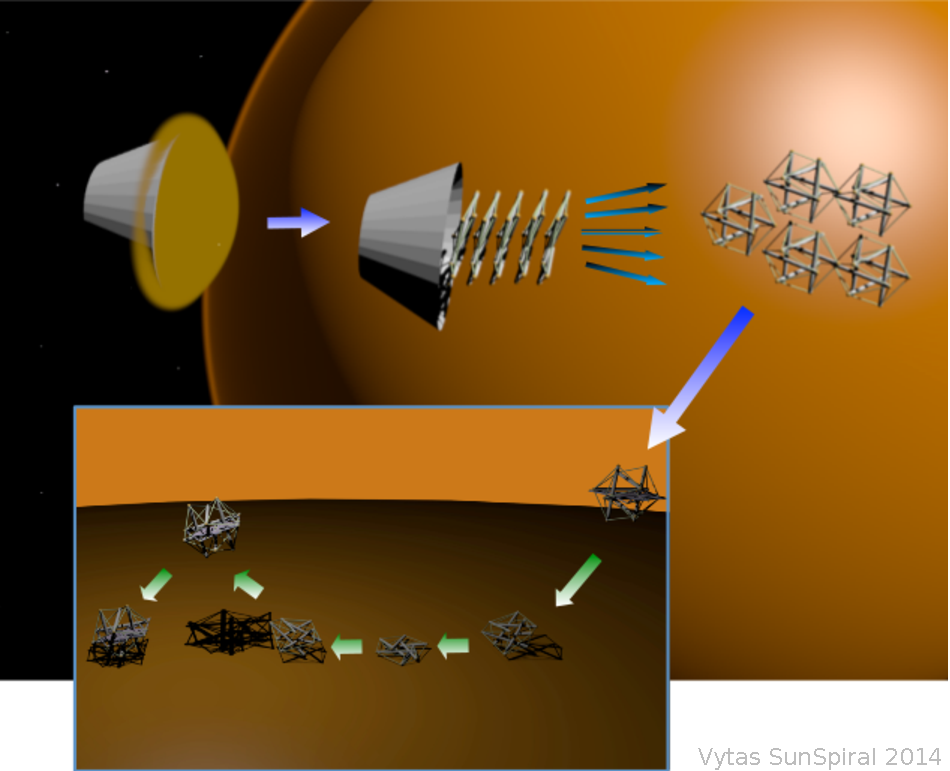
\includegraphics[width=0.5\textwidth]{tex/img/fig_aeroshell_summary} 
   \caption{{\em Tensegrity structures are composed of pure compression and tension elements. They can be lightweight, reliable, deployable, and efficient to manipulate. {\bf Mission Scenario} - Tightly packed set of tensegrities, expand, spread out, fall to surface of moon, then safely bounce on impact. The same tensegrity structure which cushioned the landing is then used for mobility to explore moons such as Titan and small asteroids.}}
   \label{fig:unpack}
\end{figure}

Tensegrity robots can facilitate an intriguing low-cost planetary exploration mission profile (see Figure~\ref{fig:unpack}) comprised of the following stages:  1) A set of tensegrity robots can be squeezed into a small launch platform; 2)  After initial atmospheric entry and ejection of the heat shield, they can automatically spring away from each other when released at their destination. 3) They bounce on impact reducing the need for final descent equipment, such as airbags; and 4) They can reorient themselves from landed position without additional reorientation hardware and efficiently move from scattered initial positions to perform sensor measurements; 5) They can survive significant falls and impacts, simplifying route planning and allowing for more aggressive exploration.

Once on the surface, tensegrity robots can perform an array of scientific analysis including soil and atmospheric composition, surface imagery and microscopic analysis. To further reduce complexity, sensors can be suspended on the interior of the tensegrity on cables attached to the nodes, or when appropriate even to the nodes themselves so that the sensors can be moved with movements of the structure itself, eliminating the need for separate sensor arms. In addition, environmental analysis can be performed in-situ at the landing site, at different local locations, or even at distant locations given a tensegrity robot's potential for efficient locomotion. The biggest advantages of this mission profile are:
\begin{enumerate}[leftmargin=.5cm]
\item The structure of the robot itself provides capability for deployment, Entry-Descent-Landing (EDL) scenarios, and mobility, reducing complexity, risk, and mass compared to using three separate systems.
\item Tensegrity robots are light-weight and can be packed tightly, reducing cost.
\item Tensegrity robots can scale to multiple tightly packed robots to increase scientific coverage and reduce risk.
%TODO do we want to keep this statement on multiple robots?
\item Flexibility and modularity of the robot design allows design reuse, reducing mission project risk.
\end{enumerate}

 \begin{figure}[h]
   \centering
   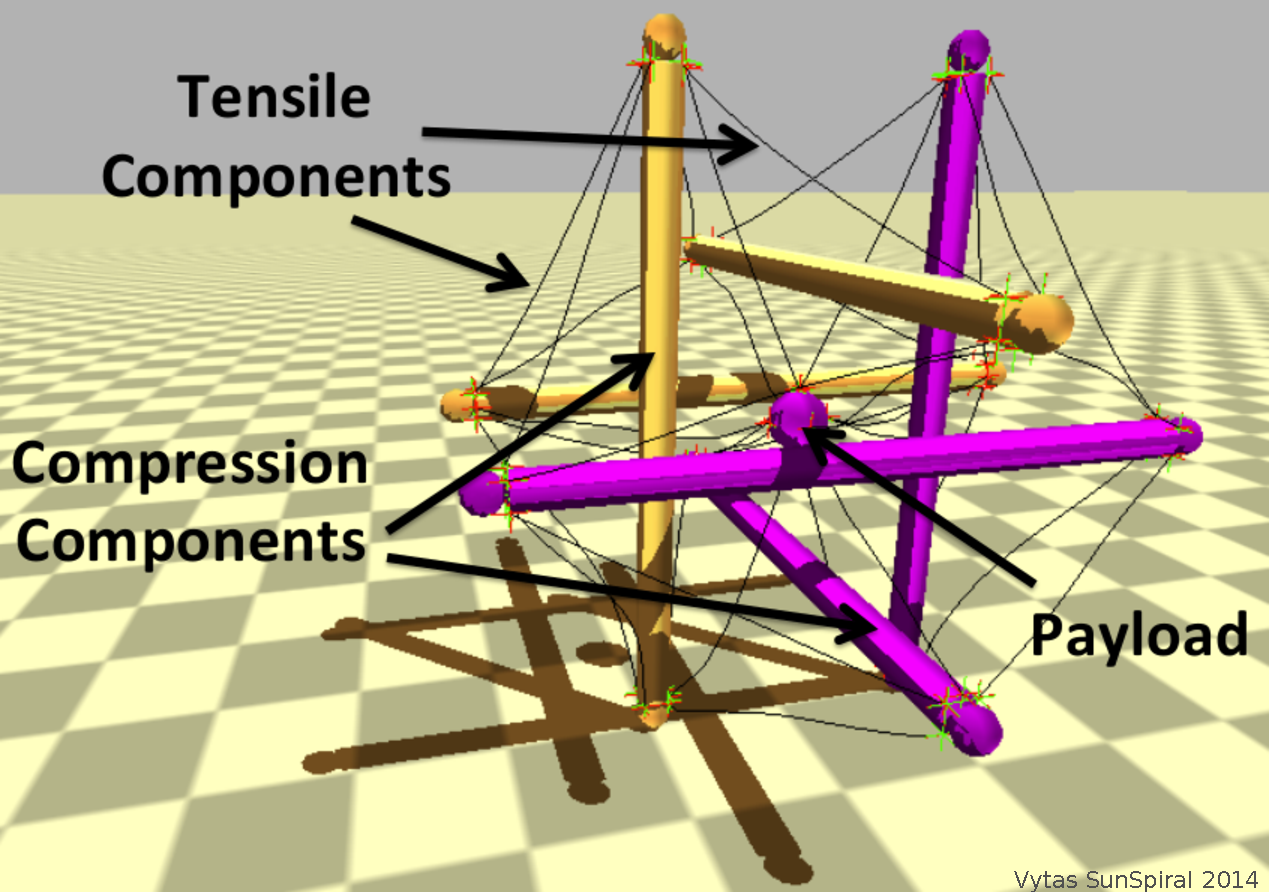
\includegraphics[width=0.5\columnwidth]{tex/img/fig_basic_diagram}
   \caption{{\em {\bf Tensegrity Structure.} Tensegrities are composed of pure tension and pure compression elements (e.g. cables and rods) as seen in this picture of a tensegrity robot from our physics based tensegrity simulator. They are light-weight, energy-efficient and robust to failures.}}
   \label{fig:basic_diagram1}
\end{figure}

\section{Goals}
\label{goal}
The main goals my project seeks to accomplish:

\begin{enumerate}[leftmargin=.5cm]
\item \textbf{Build a rolling tensegrity robot}\\
A physical hardware prototype of an untethered tensegrity robot to explore locomotion.
The robot will not only need to perform the basics for rolling, but will need to enable the next two goal items.
To achieve this, the robot will need significant mechanical power, distributed computation, and wireless communication.

\item \textbf{Open loop locomotion control}\\
Once the hardware prototype is built, an open loop control scheme will be developed.
The open loop algorithm will not change the control inputs to the system based on sensing outside of the robot.
This will demonstrate the system's ability to coordinate motion between it's distributed computation and collect data wirelessly.

\item \textbf{Closed loop "gait" control}\\
Once the system has proven the ability to locomote open loop, a closed loop algorithm will be developed.
The closed loop control will change the "gait", or locomotion pattern, of the robot to cope with sensed variations in terrain, e.g. changes in terrain grade or climbing over an obstacles.
To achieve this, research into the how much of the robot state is needed as well as various techniques to model and predict the environment by using the on board sensors.
\end{enumerate}
